%! TEX root = **/010-main.tex
% vim: spell spelllang=en:

\subsection{Decision Trees}%
\label{sub:decision-trees}
We decided that in order to find the ideal depth of the decision tree, we had to try a range of values and pick the best performing one.

We tried all values between 1 and 50 and we found out that the best performing depth was around 5. 

\begin{figure}[H]
    \centering
    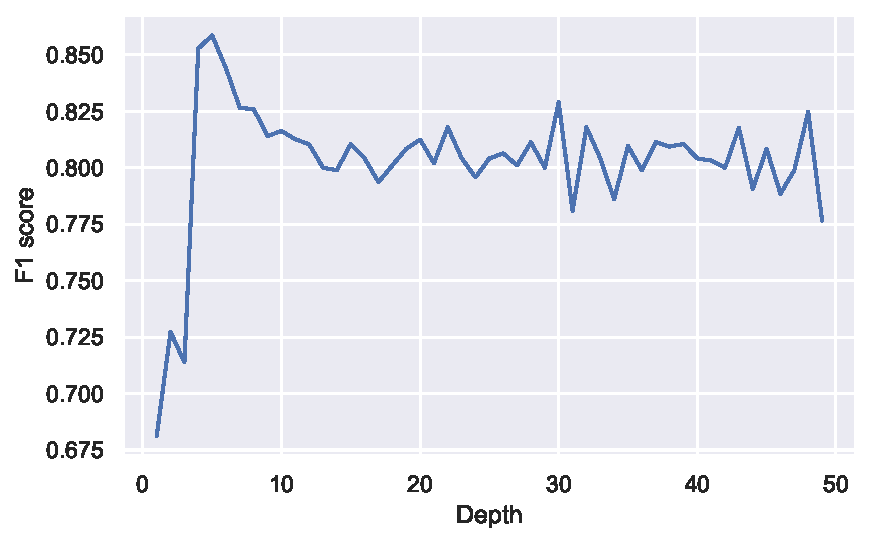
\includegraphics{decision_trees}
    \caption{decision trees accuracy depending on the depth.}%
    \label{fig:decision_trees_acc}
\end{figure}

\begin{figure}[H]
    \centering
    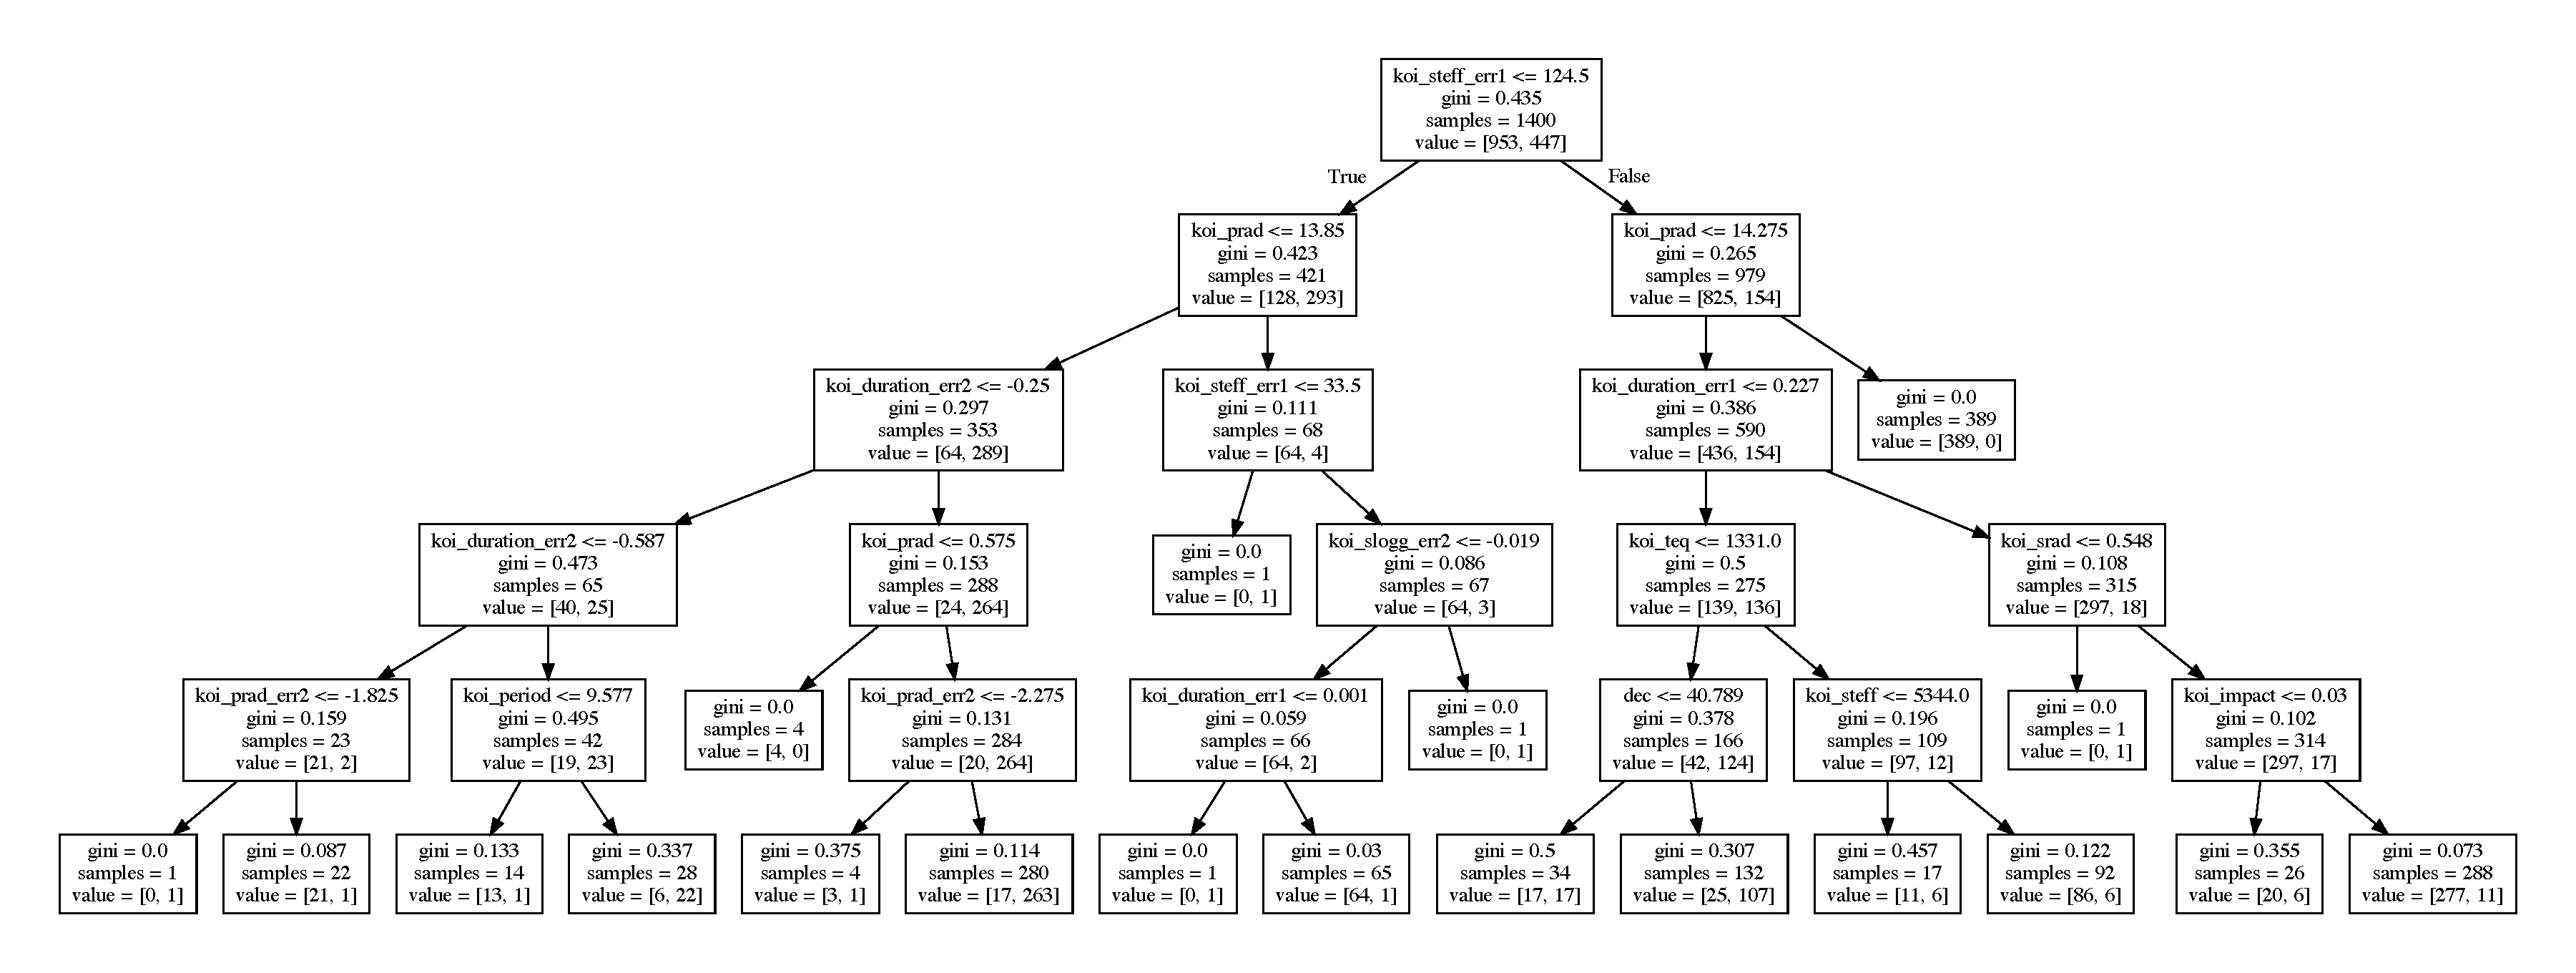
\includegraphics[width=\textwidth]{decision_tree}
    \caption{decision trees accuracy depending on the depth.}%
    \label{fig:decision_trees}
\end{figure}

% Discussion of choice of parameters used. Try to interpret the obtained DT using some examples of the validation set. 
% Show some of the most relevant rules.  Discuss how + and – examples are mixed in leaves in order to
% estimate the reliability of the tree.